本章將介紹論文中作為基礎實驗的隱藏式馬可夫模型及串接式系統(Tandem)。
由於語音辨識中所使用的隱藏式馬可夫模型是連續分佈隱藏式馬可夫模型(Continuous Hidden Markov Model; Continuous-HMM),
所以這章介紹的是連續分佈隱藏式馬可夫模型而非離散分佈隱藏式馬可夫模型(Discrete Hidden Markov Model; Discrete-HMM)。
在本章中段則介紹多層感知器的理論,
這是因為串接式系統會使用到多層感知器(Multi-Layered Perceptron; MLP)。
最後,
我們介紹串接式系統的架構。

\section{連續分佈隱藏式馬可夫模型}
  隱藏式馬可夫模型(Hidden Markov Model, HMM)被廣泛地應用於不同問題,
  現今只要是問題跟序列標籤(Sequence Tagging)或是序列分段(Seqeunce Segmentation)相關的問題,
  都有隱藏式馬可夫模型的蹤影,
  像是詞類標籤(Part-of-speech Tagging)、統計語言模型(Statistical Language Modeling)等屬於自然語言處理(Natural Language Processing; NLP)的問題。
  跟語音辨識不同的是,
  在自然語言處理的問題中,
  特徵向量多半是離散(Discrete)的,
  即特徵向量空間(Feature Vector Space)是有限可數的(Finitely Countable)。
  因此,
  隱藏式馬可夫模型中每一個狀態(State)的放射機率(Emission Probability)分佈可以用機率質量函數(Probability Mass Function)來表示,
  這種隱藏式馬可夫模型我們稱作離散分佈隱藏式馬可夫模型(Discrete Hidden Markove Model)。
  語音辨識中的特徵向量每一維則都是實數,
  也就是說特徵向量空間是不可數的(Uncountable),
  所以必須把放射機率分佈改成為機率密度函數(Probability Density Function)才能正常運作。
  由於語音辨識使用的是連續分佈隱藏式馬可夫模型,
  以下我們將用數學的語言描述它的結構、參數估測的演算法。
  
  \subsection{模型結構}
    隱藏式馬可夫模型屬於統計模型中的生成模型(Generative Model),
    這表示我們假設要建立模型的對象是經由一連串丟骰子的動作而得到的。
    \begin{algorithm} 
      \begin{algorithmic}[1]
	\STATE 上帝依照它自己的意思,創造出$M$個狀態:$\mathbf{\Omega} = \lbrace 1, 2, \ldots M\rbrace$。大自然的運行就只是在這幾個狀態間跳來跳去
	\STATE 上帝丟一顆遵守均勻分佈(Uniform Distribution)的骰子$\mathbf{\pi}$,骰子的每一面代表$M$種狀態中的一個狀態,來決定大自然一開始在哪個狀態。
	\STATE 上帝創造出一顆特別的骰子$\mathbf{A}$,骰子的每一面也是$M$個狀態中的一種,但丟出哪一面的機率是依據之前丟出的$l$種狀態是什麼。
	\STATE 上帝再創造另一顆特別的骰子$\mathbf{B}$,骰子的每一面是人類實際觀察到諸多現象的一種,這諸多現象有可能是有限可數(Finitly Countable)、無限可數(Infinitly Countable)或不可數(Uncountable)。出現哪一種現象的機率是依據現在大自然處在什麼樣的狀態。
	\FOR{$t = 1, \dots, T$}
	  \STATE 上帝丟骰子$\mathbf{A}$,來決定大自然下一個狀態是什麼狀態。 
	  \STATE 進入下一個狀態後,上帝丟骰子$\mathbf{B}$來決定人類看到的是什麼現象。
	\ENDFOR
      \end{algorithmic}
      \caption{上帝的演算法} 
      \label{alg:god}
    \end{algorithm}
    今天我們觀察到一個序列,
    我們假設這個序列是(哲學上的)上帝是經由演算法\ref{alg:god}來產生的,
    也就是我們看到的一連串現象都是由大自然對應的一系列狀態來產生。
    其中骰子$\mathbf{A}$, $\mathbf{B}$, $\mathbf{\pi}$在這裡都假設是已知。
    則我們可以用有限狀態機(Finite State Machine; FSM)來表示上帝的演算法,
    每個圓圈代表演算法中的狀態,
    而邊(Edge)則表示轉移機率。
    如圖\ref{fig:general_hmm}所示。
    (為了容易表示,這邊假設骰子$\mathbf{B}$可以表達成機率質量函數,並且假設$l = 1$)。
    \begin{figure}
      \begin{center}
	\begin{tikzpicture}[->,>=stealth',shorten >=1pt,auto,node distance=5cm,semithick]
	\tikzstyle{every state}=[fill=white,draw=black,text=black]

	\node[state]	       (A)                    {};
	\node[state]	       (B) [below left of=A]  {};
	\node[state]	       (C) [below right of=A] {};

	\path (A) edge [bend right]  node {0.1}		(B)
		  edge [bend left] node {0.2}		(C)
		  edge [loop above] node {0.7}		()
	      (B) edge [bend left] node {0.4}		(C)
		  edge [bend right] node {0.05}		(A)
		  edge [loop left]  node {0.55}		()
	      (C) edge [bend left]  node {0.3}		(A)
		  edge [bend left] node {0.3}		(B)
		  edge [loop right] node {0.4}		();
	\end{tikzpicture}
      \end{center}
      \caption{隱藏式馬可夫模型}
      \label{fig:general_hmm}
    \end{figure}

    我們下列來說明隱藏式馬可夫模型所有的參數。
    在說明之前,
    先來定義符號。
    我們用$\mathbf{X}_t$表示第$t$個時間時產生現象的隨機變數、
    而$s_t$則表示在第$t$個時間狀態的隨機變數。
    \begin{itemize}
      \item $l$:轉移到下一個狀態的機率是根據之前$l$個的狀態來決定,
	所以要將隱藏式馬可夫模型描述完整的話,
	要說成$l$階隱藏式馬可夫模型($l$-th-order Hidden Markov Model; $l$-th-order HMM),
	一般來說,
	在語音辨識或自然語言處理的問題中,
	我們用的都是一階隱藏式馬可夫模型。
	本論文從這邊開始,
	我們沒有特別說明的話,
	提及隱藏式馬可夫模型都是指一階隱藏式馬可夫模型(First-order Hidden Markov Model; First-order HMM)。

      \item $\mathbf{\Omega} = \lbrace 1, 2, \ldots, M\rbrace$:
	表示隱藏式馬可夫模型的狀態字典集(Alphabet Set)。
	同時也包含進了有限狀態機總共有$M$個狀態這項參數,
	其編號從$1$到$M$。

      \item $\mathbf{O}_W$: 
	為隱藏式馬可夫模型的現象字典集(Observation Alphabet Set)。
	這個字典集可能是有限可數(Finitly Countable)、無限可數(Infinitely Countable)、不可數(Uncountable)。
	其中不可數的現象字典集我們必須使用連續分佈隱藏式馬可夫模型才能為現象建立模型。

      \item $\mathbf{A} = \lbrace a_{ij} \rbrace$:
	即上帝演算法中的骰子$\mathbf{A}$。
	表示從給定前$l$個狀態轉移到下一個狀態的轉移機率(Transition Probability)。
	如果是一階隱藏式馬可夫模型的話,
	$\mathbf{A}$就是一個二維的矩陣(Matrix),
	其中$a_{ij}$代表由前一個狀態$i$,
	轉移到下一個狀態$j$的機率。
	即
	\begin{equation}
	  a_{ij} = P(s_t = j | s_{t-1} = i)
	\end{equation}

      \item $\mathbf{B} = \lbrace b_j(\mathbf{x}) \rbrace$:
	即上帝演算法中的骰子$\mathbf{B}$。
	代表如果現在的狀態是狀態$j$,
	產生的現象(Observation)為$\mathbf{x}$的機率,
	我們稱為放射機率(Emission Probability)。
	即
	\begin{equation}
	  b_j(\mathbf{x}) = P(X_t = \mathbf{x} | s_t = j)
	\end{equation}
	如果放射機率是機率質量函數的話,
	我們可以進一步將上式寫成
	\begin{equation}
	  b_j(o_k) = P(X_t = o_k | s_t = j)
	\end{equation}
	其中$o_k$代表現象字典集中的第$k$個字符。
	於是$\mathbf{B}$就可以表示成: (狀態數)$\times$(現象字典集大小)的一個二維矩陣。

	但假如放射機率是機率密度函數的話,
	我們就必須假設某個機率分佈家族(Probability Distribution Family)。
	一般來說,
	我們都是假設多變量混合高斯密度函數(Multivariate Gaussian Mixture Density Function)來做為我們的機率密度函數。
	它的好處是,
	只要混合數的數量足夠多,
	他就可以逼近任何連續的機率密度函數。
	所以我們假設我們有$C$個高斯密度函數
	則放射機率可以寫成下列式子:
	\begin{equation}
	  b_j(\mathbf{x}) = \sum_{k=1}^C c_{jk} N(\mathbf{x}, \mu_{jk}, \Sigma_{jk}) = \sum_{k=1}^C c_{jk} b_{jk}(\mathbf{x}) 
	\end{equation}
	其中$b_{jk}(\mathbf{x}) = N(\mathbf{x}, \mu_{jk}, \Sigma_{jk})$代表的是
	附屬於第$j$個狀態、
	平均值(Mean)向量為$\mu_{jk}$、
	共變異(Covariance)矩陣為$\Sigma_{jk}$的一個高斯密度函數,
	而$c_{jk}$是每一個元件(Component)的權重,
	必須滿足加起來為1的條件。
	\begin{equation}
	  \sum_{k=1}^C c_{jk} = 1
	\end{equation}

      \item $\mathbf{\pi} = \lbrace \pi_i \rbrace$:
	這邊的$\mathbf{\pi}$就是上帝的骰子$\mathbf{\pi}$。
	代表我們一開始從第$i$個狀態開始的機率,
	又稱為初始機率(Initial Probability)。
	可以寫成有$M$個元素一維矩陣。
    \end{itemize}

    有上述的說明,
    很明顯隱藏式馬可夫模型的參數有一些限制如下:
    \begin{align}
      &a_{ij} \geq 0, b_i(\mathbf{x}) \geq 0, \pi_i \geq 0, \forall i, j, k \\
      &\sum_{j=1}^M a_{ij} = 1	\\
      &\int_{x \in \mathbf{O}_W} b_i(\mathbf{x}) = 1 \\
      &\sum_{i=1}^M \pi_i = 1 
    \end{align}

    儘管一階隱藏式馬可夫模型可以是任意有限狀態機的形式,
    但對於序列標籤或序列分段的問題,
    我們一般是假設有限狀態機的結構是從左到右,
    即只有轉移到右邊的狀態或轉移到自己的時候轉移機率才不為零。
    其結構如圖\ref{fig:left_to_right_hmm}
    \begin{figure}
      \begin{center}
	\begin{tikzpicture}[->,>=stealth',shorten >=1pt,auto,node distance=2.8cm,semithick]
	\tikzstyle{every state}=[fill=white,draw=black,text=black]

	\node[state]	       (A)                    {1};
	\node[state]	       (B) [right of=A]	      {2};
	\node[state]	       (C) [right of=B]	      {3};
	\node[state]	       (D) [right of=C]       {4};
	\node[state]           (E) [right of=D]       {5};

	\path (A) edge              node {1.0} (B)
	      (B) edge		    node {0.4} (C)
		  edge [loop above] node {0.6} ()
	      (C) edge              node {0.5} (D)
		  edge [loop above] node {0.5} ()
	      (D) edge              node {0.1} (E)
		  edge [loop above] node {0.9} ();
	\end{tikzpicture} 
      \end{center}
      \caption{從左到右的隱藏式馬可夫模型}
      \label{fig:left_to_right_hmm}
    \end{figure}

    到目前為止,
    我們都是假設隱藏式馬可夫模型的參數是已知的,
    下一節,
    我們將說明如何從訓練語料集估測隱藏式馬可夫模型的參數。
    為了數學式子寫起來簡潔,
    我們定義:
    \begin{equation}
      \Phi = (\mathbf{A}, \mathbf{B}, \mathbf{\pi}) 
    \end{equation}
    這樣我們再寫模型參數的時候只要寫一個$\Phi$就行了,
    而不用將$\mathbf{A}, \mathbf{B}, \mathbf{\pi}$都寫出來。

  \subsection{模型參數估測}
    首先我們假設訓練語料集(Training Set)$Z$由從1開始編號的$N$個樣本點所組成,
    數學定義如下:
    \begin{equation}
	Z = \lbrace X^{(n)} \rbrace_{n=1}^{N}
    \end{equation}
    其中每個樣本點又代表一個特徵向量序列(Feature Vector Sequence),
    $(\mathbf{X}_i^{(n)})$表示第$n$個樣本點的第$i$個特徵向量。

    我們這邊用最大相似度估測法(Maximum Likelihood Estimation)來估測參數,
    首先$N$個樣本點的相似度(Likelihood)可以寫成下式:
    \begin{equation}
      \prod_{n=1}^N P(X^{(n)}; \Phi)
    \end{equation}
    對相似度取對數可以幫助我們運算,
    於是對數相似度(Log-Likelihood)如下:
    \begin{equation}
      l(\Phi) = \sum_{n=1}^N \log P(X^{(n)} ; \Phi)
    \end{equation}

    我們希望將連續式隱藏式馬可夫模型的參數調適(Fit)到訓練語料集,
    但由於連續式隱藏式馬可夫模型的狀態是隱藏變數(Hidden Variable),
    所以直接用最大相似度估測法有困難,
    我們改用期望值最大法(Expectation Maximization)來估測參數。
    首先,
    將對數相似度重寫如下:
    \begin{equation}
      \begin{split}
	l(\Phi) 
	&= \sum_{n=1}^N \log P(X^{(n)} ; \Phi) \\
	&= \sum_{n=1}^N \log \left( \sum_{S^{(n)}} P(X^{(n)}, S^{(n)}; \Phi) \right) \\
	&= \sum_{n=1}^N \log \left( \sum_{S^{(n)}} \sum_{K^{(n)}} P(X^{(n)}, S^{(n)}, K^{(n)}; \Phi) \right) \\
      \end{split}
    \end{equation}

    接著,
    按照期望值最大法,
    我們假設$Q_n(S^{(n)}, K^{(n)})$是某個機率分佈,
    其中$S^{(n)}$是代表狀態序列(State Sequence)的隱藏變數,
    $K^{(n)}$則代表混合高斯模型中所使用的第幾個高斯密度函數所形成序列的隱藏變數。
    因此我們有
    \begin{align}
      &\sum_{S^{(n)}} \sum_{K^{(n)}} Q_n(S^{(n)}, K^{(n)}) = 1 \\
      &Q_n(S^{(n)}, K^{(n)}) \geq 0
    \end{align}
    根據詹氏不等式(Jensen's Inequality),
    推導對數相似度的下限(Lower Bound):
    \begin{equation}
      \begin{split}
	l(\Phi) 
	&= \sum_{n=1}^N \log \left( \sum_{S^{(n)}} \sum_{K^{(n)}} P(X^{(n)}, S^{(n)}, K^{(n)}; \Phi) \right) \\
	&= \sum_{n=1}^N \log \left( \sum_{S^{(n)}} \sum_{K^{(n)}} Q_n(S^{(n)}, K^{(n)}) \frac{P(X^{(n)}, S^{(n)}, K^{(n)}; \Phi)}{Q_n(S^{(n)}, K^{(n)})} \right) \\
	&\geq \sum_{n=1}^N \sum_{S^{(n)}} \sum_{K^{(n)}} Q_n(S^{(n)}, K^{(n)}) \log \left( \frac{P(X^{(n)}, S^{(n)}, K^{(n)}; \Phi)}{Q_n(S^{(n)}, K^{(n)})} \right) \\
	&= \sum_{n=1}^N \sum_{S^{(n)}} \sum_{K^{(n)}} Q_n(S^{(n)}, K^{(n)}) \log \left( P(X^{(n)}, S^{(n)}, K^{(n)}; \Phi) \right) \\
	&- \sum_{n=1}^N \sum_{S^{(n)}} \sum_{K^{(n)}} Q_n(S^{(n)}, K^{(n)}) \log \left( Q_n(S^{(n)}, K^{(n)}) \right) 
	\label{eq:jensen_lower_bound}
      \end{split}
    \end{equation}
    為了要讓下限盡量緊一些,
    讓詹式不等式的等號成立是最好。
    這表示必須讓隨機變數等於某個常數的機率為1。
    如下:
    \begin{equation}
	\frac{P(X^{(n)}, S^{(n)}, K^{(n)}; \Phi)}{Q_n(S^{(n)}, K^{(n)})} = c
    \end{equation}
    所以
    \begin{equation}
	P(X^{(n)}, S^{(n)}, K^{(n)}; \Phi) \propto Q_n(S^{(n)}, K^{(n)})
    \end{equation}
    再加上$\sum_{S^{(n)}} \sum_{K^{(n)}} Q_n(S^{(n)}, K^{(n)}) = 1$的限制,
    因此
    \begin{equation}
      \begin{split}
	Q_n(S^{(n)}, K^{(n)})
	&= \frac{P(X^{(n)}, S^{(n)}, K^{(n)}; \Phi)}{\sum_{S^{(n)}} \sum_{K^{(n)}} P(X^{(n)}, S^{(n)}, K^{(n)}; \Phi)} \\
	&= \frac{P(X^{(n)}, S^{(n)}, K^{(n)}; \Phi)}{P(X^{(n)}; \Phi)} \\
	&= P(S^{(n)}, K^{(n)} | X^{(n)}; \Phi) 
      \end{split}
    \end{equation}
    所以我們知道,
    當$Q_n(S^{(n)}, K^{(n)}) = P(S^{(n)}, K^{(n)} | X^{(n)}; \Phi)$時下限是最緊的。

    注意到式子\ref{eq:jensen_lower_bound}中後面一項在一個循環之中是不變的。
    \begin{equation}
      \sum_{n=1}^N \sum_{S^{(n)}} \sum_{K^{(n)}} Q_n(S^{(n)}, K^{(n)}) \log \left( Q_n(S^{(n)}, K^{(n)}) \right) 
    \end{equation}
    所以我們只需要最大化
    \begin{equation}
      \sum_{n=1}^N \sum_{S^{(n)}} \sum_{K^{(n)}} Q_n(S^{(n)}, K^{(n)}) \log \left( P(X^{(n)}, S^{(n)}, K^{(n)}; \hat{\Phi}) \right) \\ 
    \end{equation}
    其中,
    為了避免混淆(我們接下來要做最大化,只有原始的機率分佈參數需要變動),
    我們這邊在$P(X^{(n)}, S^{(n)}, K^{(n)}; \hat{\Phi})$用$\hat{\Phi}$來代替$\Phi$。

    我們將取期望值步驟中得到的$Q_i$代入:
    \begin{equation}
      \begin{split}
	&\sum_{n=1}^N \sum_{S^{(n)}} \sum_{K^{(n)}} Q_n(S^{(n)}, K^{(n)}) \log \left( P(X^{(n)}, S^{(n)}, K^{(n)}; \hat{\Phi}) \right) \\
	&= \sum_{n=1}^N \sum_{S^{(n)}} \sum_{K^{(n)}} \frac{P(X^{(n)}, S^{(n)}, K^{(n)}; \Phi)}{P(X^{(n)}; \Phi)} \log \left( P(X^{(n)}, S^{(n)}, K^{(n)}; \hat{\Phi}) \right) 
      \end{split}
    \end{equation}
    由於我們假設的是有限狀態機的結構,
    因此$P(X^{(n)}, S^{(n)}, K^{(n)} | \hat{\Phi})$可以寫成:
    \begin{equation}
      \begin{split}
	P(X^{(n)}, S^{(n)}, K^{(n)} | \hat{\Phi}) 
	&= \prod_{t=1}^T \hat{a}_{s_{t-1} s_t} \hat{b}_{s_t} (X^{(n)}_{t})\\
	&= \prod_{t=1}^T \hat{a}_{s_{t-1} s_t} \hat{b}_{s_t k_t} (X^{(n)}_{s_t}) \hat{c}_{s_t k_t} 
      \end{split}
    \end{equation}
    對上式取對數,
    得到
    \begin{equation}
     \log P(X^{(n)}, S^{(n)}, K^{(n)} | \hat{\Phi}) = \sum_{t=1}^T \log \hat{a}_{s_{t-1} s_t} + \sum_{t=1}^T \log \hat{b}_{s_t k_t} (x_t) + \sum_{t=1}^T \log \hat{c}_{s_t k_t}
    \end{equation}
    取對數後能夠拆解這項性質扮演了關鍵角色,
    這代表式子\ref{eq:jensen_lower_bound}也可以拆解。
    \begin{equation}
      \begin{split}
	&\sum_{n=1}^N \sum_{S^{(n)}} \sum_{K^{(n)}} P(S^{(n)}, K^{(n)} | X^{(n)}; \Phi) \log P(X^{(n)}, S^{(n)}, K^{(n)} | \hat{\Phi}) \\
	&= \sum_{n=1}^N \sum_{i=1}^{M} \sum_{j=1}^{M} \sum_{t=1}^T P(s_{t-1} = i, s_t = j | X^{(n)}; \Phi) \log \hat{a}_{ij} \\
	&+ \sum_{n=1}^N \sum_{j=1}^M \sum_{k=1}^C \sum_{t=1}^T P(s_t = j, k_t = k | X^{(n)}; \Phi) \log \hat{b}_{jk} (x^{(n)}_t) \\
	&+ \sum_{n=1}^N \sum_{j=1}^M \sum_{k=1}^C \sum_{t=1}^T P(s_t = j, k_t = k | X^{(n)}; \Phi) \log \hat{c}_{jk} \\
      \end{split}
    \end{equation}
    上面的式子可拆解代表我們做微分等於零的動作來最大化的時候,
    可以分別對每一項做最大化。
    更重要的是,
    第一項跟第三項的形式都是
    \begin{equation}
      F(x) = \sum_i y_i \log x_i
    \end{equation}
    且$\sum_i x_i = 1$。

    這種形式用拉氏乘數法(Lagrange Multiplier)就可以知道解是
    \begin{equation}
      x_i = \frac{y_i}{\sum_i y_i}
    \end{equation}
    因此第一項跟第三項的解分別為
    \begin{align}
      \hat{a}_{ij} = \frac{ \sum_{n=1}^N \sum_{t=1}^T \gamma^{(n)}_t (i,j) }{ \sum_{k=1}^M \sum_{n=1}^N \sum_{t=1}^T \gamma^{(n)}_t (i,j) } \\
      \hat{c}_{jk} = \frac{ \sum_{n=1}^N \sum_{t=1}^T \xi^{(n)}_t (j,k) }{ \sum_{k=1}^C \sum_{n=1}^N \sum_{t=1}^T \xi^{(n)}_t (j,k) }	  
    \end{align}
    其中$\xi^{(n)}_t (j, k)$代表
    \begin{equation}
      \xi^{(n)}_t (j, k) = P(s_t = j, k_t = k | X^{(n)}; \Phi)	
    \end{equation}  
    而$\gamma^{(n)}_t (i, j)$代表
    \begin{equation}
      \gamma^{(n)}_t (i, j) = P(s_{t-1} = i, s_t = j | X^{(n)}; \Phi)
    \end{equation}
    唯一比較複雜的是第二項,
    因為它又依賴於$\lbrace \mu_{jk}, \Sigma_{jk} \rbrace$。
    因此在做拉式乘數法的時候必須要使用鏈鎖法則(Chain Rule)。
    經過一連串運算,
    我們可以得到
    \begin{equation}
      \begin{split}
	\hat{\mu}_{jk} 
	&= \frac{ \sum_{t=1}^T P(s_t = j, k_t = k | X^{(n)} ;\Phi) x_t }{ \sum_{t=1}^T P(s_t = j, k_t = k | X^{(n)}; \Phi)} \\ 
	&= \frac{ \sum_{t=1}^T \xi^{(n)}_t(j, k) x_t }{ \sum_{t=1}^T \xi^{(n)}_t (j, k) } \\
      \end{split}
    \end{equation}

    \begin{equation}
      \begin{split}
	\hat{\Sigma}_{jk} 
	&= \frac{ \sum_{t=1}^T P(s_t = j, k_t = k | X^{(n)}; \Phi) (x_t - \hat{\mu}_{jk})(x_t - \hat{\mu}_{jk})^T }{ \sum_{t=1}^T P(s_t = j, k_t = k | X^{(n)}; \Phi) } \\
	&= \frac{ \sum_{t=1}^T \xi^{(n)}_t (j,k) (x_t - \hat{\mu}_{jk})(x_t - \hat{\mu}_{jk})^T }{ \sum_{t=1}^T \xi^{(n)}_t (j,k) } \\
      \end{split}
    \end{equation}

    \begin{algorithm}
      \caption{前向演算法(Forward Algorithm)}
      \label{alg:forward}
      \begin{algorithmic}[1]
	\FOR{$i = 1, \dots M$}
	  \STATE $\alpha_1(i) = \pi_i b_i(X_1)$ 
	\ENDFOR
	\FOR{$t = 2, \dots, T$}
	  \FOR{$i = 1, \dots, M$}
	    \STATE $\alpha_t(j) = \left[ \sum_{i=1}^M \alpha_{t-1}(i) a_{ij} \right] b_j(X_t)$ 
	  \ENDFOR
	\ENDFOR
	\STATE $P(X; \Phi) = \sum_{i=1}^M \alpha_T(i)$
      \end{algorithmic}
    \end{algorithm}
   
    現在最大的問題是,
    我們如何能夠將$\xi^{(n)}_t (j, k)$和$\gamma^{(n)}_t (i, j)$算出來。
    這就是波氏-維氏演算法(Baum-Welch Algorithm)發揮用處的地方。
    波氏-維氏演算法由演算法\ref{alg:forward}及演算法\ref{alg:backward}所構成。
    其中前向演算法(演算法\ref{alg:forward}可以幫助我們出$\alpha_t(i)$,
    代表的意思是
    \begin{equation}
      \alpha_t(i) = P(X_{1}^{t} | s_t = i; \Phi)
    \end{equation}
    而後向演算法(演算法\ref{alg:backward}可以幫助我們算出$\beta_t(i)$,
    代表的意思是
    \begin{equation}
      \beta_t(i) = P(X_{t+1}^T | s_t = i; \Phi)
    \end{equation}
    有了$\alpha_t(i)$跟$\beta_t(i)$, 
    我們就可以用下列式子算出$\xi^{(n)}_t (j, k)$和$\gamma^{(n)}_t (i, j)$。
    \begin{align}
      & \gamma^{(n)}_t (i, j) = \frac{ \sum_{k=1}^C \alpha_{t-1} (i) a_{ij} c_{jk} b_{jk} (x_t) \beta_t(j) }{ \sum_{i=1}^M \alpha_T(i) } \\ 
      & \xi^{(n)}_t (j, k) = \frac{ \sum_{i=1}^M \alpha_{t-1} (i) a_{ij} c_{jk} b_{jk} (x_t) \beta_t(j) }{ \sum_{i=1}^M \alpha_T(i) }  
    \end{align}
    將$\xi^{(n)}_t (j, k)$和$\gamma^{(n)}_t (i, j)$代入之前更新參數的式子,
    便可以得到新的一組參數。
    \begin{algorithm}
      \caption{後向演算法(Backward Algorithm)}
      \label{alg:backward}
      \begin{algorithmic}[1]
	\STATE $\beta_T(i) = \frac{1}{M}$ 
	\FOR{$t = T-1, \dots, 1$}
	  \FOR{$i = 1, \dots, M$}
	    \STATE $\beta_t(i) = \left[ \sum_{j=1}^M a_{ij} b_j(X_{t+1}) \beta_{t+1}(j) \right]$
	  \ENDFOR
	\ENDFOR
      \end{algorithmic}
    \end{algorithm}

\section{多層感知器(Multi-Layered Perceptron)}
  早期機器學習的研究者們受到神經科學(Neuro Science)的啟發,
  試著建立一個模型來模仿神經元突觸的行為。
  如圖\ref{fig:neuron},
  一個神經元的作用就是將它接受到的訊號,
  經過某種轉換後,
  再傳給下一個神經元。
  \begin{figure}
    \centering
    \subfloat[人體的神經元]{\label{fig:neuron}\includegraphics[scale=1.0]{images/neuron.pdf}}
    \subfloat[數學的神經元]{\label{fig:artificial_neuron}\includegraphics[scale=2.0]{images/math_neuron.pdf}}
  \end{figure}
  這跟數學上的函數其實是一樣的,
  因此我們只要想辦法找出一個函數符合真實神經元的情況也許就可以模擬其行為。
  但實際上我們並不知道那是什麼樣的函數。
  只好假設它是輸入向量線性組合的某個轉換,
  寫成數學式子如下:
  \begin{equation}
    F(\mathbf{x}) = \varphi \left( \sum_i w_i x_i \right)
  \end{equation}
  其中$\mathbf{x}$是輸入訊號,$\varphi$是某個數學轉換(Transformation),而$w_i$是線性組合的加權(Weight)。
  如果將上面的概念畫成圖,就像圖\ref{fig:artificial_neuron}一般。
  很明顯這樣的結構太簡單,
  無法提供我們強而有力的模型。
  但我們可以將這些小的神經元串接起來來得到一個強力的模型。
  而這樣串接起來的模型我們稱作類神經網路(Neuro Network)。
  但如果串接的結構太複雜,
  又超出我們可以計算的能力。
  所以我們限制其串接的結構,
  規定串接的時候只能串接成一個無迴路(Acyclic)的類神經網路,
  並給予它另一個名稱,
  叫做多層感知器(Multi-Layered Perceptron),
  又名前向遞推類神經網路(Feed-Forward Neural Network),
  為類神經網路的一個子集。
  其結構如圖\ref{fig:mlp}。
  經常的用途是對付分類(Classification)問題、迴歸(Regression)問題,或將高維的特徵向量轉換到較低維度的向量。
  \def\layersep{2.5cm}
  \begin{figure}
    \begin{center}
      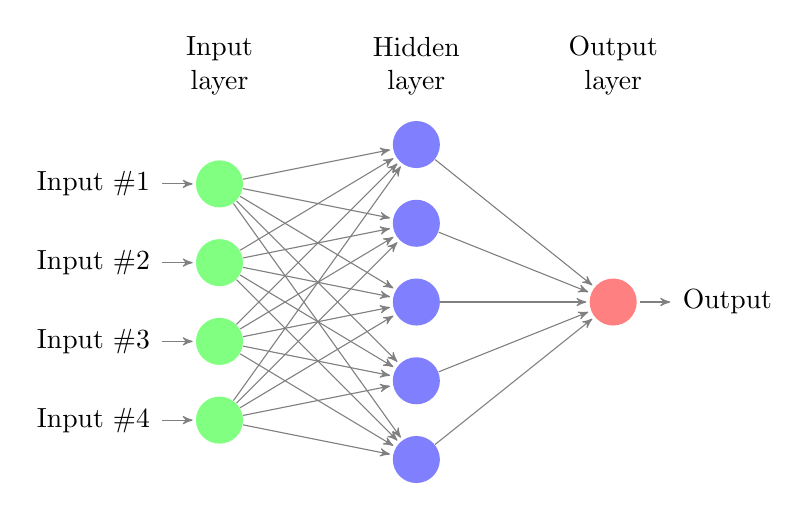
\begin{tikzpicture}[shorten >=1pt,->,draw=black!50, node distance=\layersep]
	  \tikzstyle{every pin edge}=[<-,shorten <=1pt]
	  \tikzstyle{neuron}=[circle,fill=black!25,minimum size=17pt,inner sep=0pt]
	  \tikzstyle{input neuron}=[neuron, fill=green!50];
	  \tikzstyle{output neuron}=[neuron, fill=red!50];
	  \tikzstyle{hidden neuron}=[neuron, fill=blue!50];
	  \tikzstyle{annot} = [text width=4em, text centered]

	  % Draw the input layer nodes
	  \foreach \name / \y in {1,...,4}
	  % This is the same as writing \foreach \name / \y in {1/1,2/2,3/3,4/4}
	      \node[input neuron, pin=left:Input \#\y] (I-\name) at (0,-\y) {};

	  % Draw the hidden layer nodes
	  \foreach \name / \y in {1,...,5}
	      \path[yshift=0.5cm]
		  node[hidden neuron] (H-\name) at (\layersep,-\y cm) {};

	  % Draw the output layer node
	  \node[output neuron,pin={[pin edge={->}]right:Output}, right of=H-3] (O) {};

	  % Connect every node in the input layer with every node in the
	  % hidden layer.
	  \foreach \source in {1,...,4}
	      \foreach \dest in {1,...,5}
		  \path (I-\source) edge (H-\dest);

	  % Connect every node in the hidden layer with the output layer
	  \foreach \source in {1,...,5}
	      \path (H-\source) edge (O);

	  % Annotate the layers
	  \node[annot,above of=H-1, node distance=1cm] (hl) {Hidden layer};
	  \node[annot,left of=hl] {Input layer};
	  \node[annot,right of=hl] {Output layer};
      \end{tikzpicture}
    \end{center}
    \caption{多層感知器}
    \label{fig:mlp}
  \end{figure}

  一般來講,
  如果是在解二元分類問題(Binary Classification)或是單元迴歸問題(Univariate Regression)的時候,
  我們設定輸出的向量就是一維的實數向量。
  如果是分類問題就取一個門檻(Threshold),
  高過門檻就是某一個分類,
  低於門檻就是另一個分類。
  如果是迴歸問題就直接使用這個實數當作我們的預測值。

  當解的問題改成多元分類問題或多元迴歸問題時,
  我們可以增加輸出向量的維數為要分類的類別數來解決問題,
  而用來估測模型參數的演算法並不會需要更動。
  
  以下,
  我們用數學的語言來描述多層感知器模型。
  
  \subsection{數學定義}
  為了方便說明模型的架構,
  這邊假設我們希望建立模型的函數是$f: \mathbb{R}^d \rightarrow \mathbb{R}$,
  即輸入的向量為$d$維,輸出的向量是一維。
  而我們建立模型的函數為$g$,
  我們希望$g$跟$f$越相近越好。

  則我們定義我們的前向遞推類神經網路如下:
  網路由$L$層串接起來的神經元(Neuron)們所組成,
  第$l$($1 \leq l \leq L$)層總共有$d^{(l)}$個神經元,
  將$d^{(l-1)}$個輸入接成$d^{(l)}$個輸出,
  這樣的結構表示第$l-1$層的輸出就是第$l$層的輸入。
  (注意如果是有跳層情況的網路,也可以重新寫成第$l$層的輸入從第$l-1$層輸出來的形式,
  所以定義由無迴路性質刻畫是正確的)。
  由以上定義,
  我們知道整個系統的輸入維度為$d^{(0)} = d$,
  而整個系統的輸出維度為$d^{(L)} = 1$。

  接著,
  我們再定義第$l$層的輸入為$x_i^{(l-1)}, (1 \leq i \leq d^{(l-1)})$、
  輸出為$x_j^{(l)}, (1 \leq j \leq d^{(l)})$。
  而第$l$層的加法權重為$w_{ij}^{(l)}, (1 \leq l \leq L, 0 \leq i \leq d^{(l-1)}, 1 \leq j \leq d^{(l)})$
  則第$l$層中的第$j$個神經元的轉換函數可定義為
  \begin{equation}
    x_j^{(l)} = \varphi \left( \sum_{i=0}^{d^{(l-1)}} w_{ij}^{(l)} x_i^{(l-1)} \right)
  \end{equation}
  其中$\varphi(s) = \tanh(s) = \frac{e^s - e^{-s}}{e^s + e^{-s}}$。

  為了後面演算法的推導方便,
  我們定義一個輔助變數$s_j^{(l)}$將神經元函數中線性的部份跟非線性的部份分開來。
  \begin{align}
    &s_j^{(l)} = \sum_{i=0}^{d^{(l-1)}} w_{ij}^{(l)} x_i^{(l-1)} \\
    &x_j^{(l)} = \varphi(s_j^{(l)})
  \end{align}
  假設模型的參數為已知,
  則使用類神經網路來計算函數$g(\mathbf{x})$的預測值便可以如下操作:
  將輸入向量$\mathbf{x}$的每一維分別擺到$x_1^{(0)}, \ldots x_{d^(0)}^{(0)}$,
  再從第一層開始一一按照上面的神經元函數計算這一層的輸出,
  直到第$L$層為止。
  則最後我們便將$x_1^{(L)}$當作$g(\mathbf{x})$輸出的值。

  \subsection{模型參數估測}
  有了前一節定義的多層感知器結構,
  這一節將探討如何利用訓練集$Z = \lbrace (\mathbf{x}_n, y_n) \rbrace_{n=1}^{N}$,
  來估計多層感知器模型的參數。

  為了要衡量我們得到的參數究竟讓模型是否更貼近我們希望建立模型的函數,
  我們需要一個錯誤衡量函數(Error Function)。
  一般來講,
  在訓練多層感知器的錯誤衡量函數都是
  \begin{equation}
    E_n(w) = (g(\mathbf{x}_n) - y_n)^2
  \end{equation}
  用二次項的好處就是可以微分,
  方便我們使用做最佳化(Optimization)的時候使用梯度下降法(Gradient Decent)。

  在這邊我們使用一種在實做上比較容易的一種梯度下降法 -- 隨機梯度下降法(Stochastic Gradient Decent)來做最佳化,
  因此我們需要計算$\frac{\partial E_n}{\partial w_{ij}^{(l)}}, 0 \leq i \leq d^{(l-1)}, (1 \leq j \leq d^{(l)}, 1 \leq l \leq L)$。
  一旦我們有了以上梯度,
  則我們可以應用隨機梯度下降法來修正權重。
  \begin{equation}
    w_{ij}^{(l)} \leftarrow w_{ij}^{(l)} - \eta \frac{\partial E_n}{\partial w_{ij}^{(l)}}
  \end{equation}
  其中$\eta$是學習速率,
  隨機梯度下降法只要執行足夠多次更新,
  就可以得到一組滿意的參數。
  \begin{algorithm}
    \caption{隨機梯度下降演算法(Stochastic Gradient Decent Algorithm)}
    \label{alg:stochastic_gradient_decent}
    \begin{algorithmic}[1]
      \STATE 視問題將$w^{(0)}$初始化為0或一組亂數。
      \FOR{$t = 1, 2, \dots, T$}
	\STATE $w^{(t)} \leftarrow w^{(t-1)} - \eta \nabla E(w^{(t-1)})$
      \ENDFOR
    \end{algorithmic}
  \end{algorithm}
  所以主要的問題是,
  是否有方法讓我們可以快速地算出$\frac{\partial E_n}{\partial w_{ij}^{(l)}}$。
  這便是我們下面要講的後向推進演算法(Backpropagation Algorithm)的目的。

  假設我們已經執行了一遍前向遞推來計算出對應訓練範例的輸出,
  在這過程中,
  注意到輔助變數$x_j^{(l)}$跟$s_j^{(l)}$已經被計算出來。
  則由於$w_{ij}^{(l)}$只透過$s_j^{(l)}$來影響輸出,
  根據鏈鎖法則(Chain Rule),
  我們有
  \begin{equation}
    \frac{\partial E_n}{\partial w_{ij}^{(l)}} = \frac{\partial E_n}{\partial s_j^{(l)}} \times \frac{\partial s_j^{(l)}}{\partial w_{ij}^{(l)}}
  \end{equation}

  其中$\frac{\partial s_j^{(l)}}{\partial w_{ij}^{(l)}} = x_i^{(l-1)}$是已經計算出來的值。
  所以只剩下如何計算$\frac{\partial E_n}{\partial s_j^{(l)}}$的問題。
  先定義$\delta_j^{(l)} = \frac{\partial E_n}{\partial s_j^{(l)}}$。
  則在最後一層$l = L$的時候,
  我們有$E_n = (x_1^{(L)} - y)^2$,
  因此我們能計算$\delta_1^{(L)}$
  \begin{equation}
    \delta_1^{(L)} = \frac{\partial E_n}{\partial s_j^{(l)}} 
    = \frac{\partial E_n}{\partial x_1^{(l)}} \times \frac{\partial x_1^{(L)}}{\partial s_1^{(l)}}
  \end{equation}
  其中$\frac{\partial E_n}{\partial x_1^{(l)}} = 2(x_1^{(L)} - y)$、
  $\frac{\partial x_1^{(L)}}{\partial s_1^{(l)}} = \varphi^{'}(s_1^{(L)})$。
  因此我們有了遞迴的初始條件。
  我們可以利用遞迴來算第$l-1$的$\delta_j^{(l-1)}$
  \begin{equation}
    \begin{split}
      \delta_i^{(l-1)} 
      &= \frac{\partial E_n}{\partial s_i^{(l-1)}} \\
      &= \sum_{j=1}^{d^{(l)}} \frac{\partial E_n}{\partial s_j^{(l)}} \times 
      \frac{\partial s_j^{(l)}}{\partial x_i^{(l-1)}} \times
      \frac{\partial x_i^{(l-1)}}{\partial s_i^{(l-1)}} \\
      &= \sum_{j=1}^{d^{(l)}} \delta_j^{(l)} \times w_{ij}^{(l)} \times \varphi^{'}(s_i^{(l-1)})
    \end{split}
  \end{equation}
  其中$\varphi^{'}(s) = 1 - \varphi^2(s)$、
  $\varphi(s_i^{(l)}) = x_i^{(l)}$
  因此$\delta_i^{(l-1)}$可以遞迴地表示成如下:
  \begin{equation}
    \delta_i^{(l-1)} = \left( 1 - (x_i^{(l-1)})^2 \right) \sum_{j=1}^{d^{(l)}} w_{ij}^{(l)} \delta_j^{(l)}
  \end{equation}
  以上的式子中的變數都在前向遞推時能算出來,
  因此我們藉由後向推進演算法就可以算出所有的$\delta$。
  有了$\delta$,我們就可以算出錯誤對權重的梯度。
  因此,
  我們可以做隨機梯度下降法來最佳化。

\section{串接式聲學模型(Tandem)}
  \usetikzlibrary{calc,trees,positioning,arrows,chains,shapes.geometric,%
      decorations.pathreplacing,decorations.pathmorphing,shapes,%
      matrix,shapes.symbols}

  \tikzset{
  >=stealth',
    punktchain/.style={
      rectangle, 
      rounded corners, 
      % fill=black!10,
      draw=black, very thick,
      text width=10em, 
      minimum height=3em, 
      text centered, 
      on chain},
    line/.style={draw, thick, <-},
    element/.style={
      tape,
      top color=white,
      bottom color=blue!50!black!60!,
      minimum width=8em,
      draw=blue!40!black!90, very thick,
      text width=10em, 
      minimum height=3.5em, 
      text centered, 
      on chain},
    every join/.style={->, thick,shorten >=1pt},
    decoration={brace},
    tuborg/.style={decorate},
    tubnode/.style={midway, right=2pt},
  }

  \begin{figure}
    \begin{tikzpicture}
    [node distance=.8cm,
    start chain=going below,]
	\node (asym) [punktchain ]  {多層感知器};
	\begin{scope}[start branch=venstre,
	  %We need to redefine the join-style to have the -> turn out right
	  every join/.style={->, thick, shorten <=1pt}, ]
	  \node[punktchain, on chain=going left, join=by {<-}]
	      (risiko) {抽取特徵向量};
	\end{scope}
	\begin{scope}[start branch=abc,]
	\node (finans) [punktchain, on chain=going right, join=by {->}] {事後機率解碼器};
	\end{scope}
    \node[punktchain, join,] (kerker) {主成份分析法};
    \node[punktchain, join,] (disk) {隱藏式馬可夫程式集混合高斯模型};
    \node[punktchain, join,] (makro) {隱藏馬可夫程式集解碼器};
    % Now that we have finished the main figure let us add some "after-drawings"
    %% First, let us connect (finans) with (disk). We want it to have
    %% square corners.
    %\draw[|-,-|,->, thick,] (finans.south) |-+(0,-1em)-| (disk.north);
    \end{tikzpicture}
    \label{fig:tandem_flow_chart}
    \caption{串接式系統流程圖}
  \end{figure}
  串接式系統(Tandem)\cite{HermanskyTandem}整體的架構如圖\ref{fig:tandem_flow_chart}。
  如果瞭解原本隱藏式馬可夫模型的系統架構的話,
  串接式系統其實很容易瞭解。
  它等於是將原本餵進隱藏式馬可夫模型的特徵向量做過一次轉換,
  再當作另一種特徵向量餵進隱藏式馬可夫模型。
  而這種轉換就是用多層感知器加上主成分分析法(Pricipal Component Analysis; PCA)來達成。
  
  整體過程如下:
  首先先將原本用來訓練隱藏式馬可夫模型的訓練資料,
  對每個音框都標上對應正確的次字元標籤
  (一般來講,就是音素標籤),
  來作為訓練多層感知器的訓練資料集。
  而這裡多層式感知器的用途,
  是輸入一個音框及其鄰近音框,
  輸出這個音框屬於某個音素的事後機率。
  因此,
  多層感知器的輸入維度為特徵向量的維度乘上一個窗戶長
  (一般取現在這個音框加上前後四個音框,共九個音框),
  輸出維度為次字元標籤的數量,
  一般使用在串接式系統的多層感知器都是三層,
  扣掉第一層、第三層為輸入、輸出,
  真正決定多層感知器力量是第二層的神經元數量,
  在做串接式系統的時候多半取1000左右。

  有了音框上次字元(Subword)的事後機率,
  一種選擇是直接對這串事後機率向量做解碼,
  這樣的架構稱為混合式系統(Hybrid System)。
  但根據赫氏(Hermansky)所述\cite{HermanskyTandem},
  由於次字元的標籤數多半在30個到50個之間,
  也就是說多層感知器輸出的向量維度也跟原本的語音特徵向量維度差不多,
  這樣對辨識結果並沒有特別的好處。

  由於事後機率的分佈擁有非常偏斜(Skew)的特性,
  因此我們將事後機率再取上一個對數(Log),
  將他轉到另一個空間去。
  轉換之後的空間讓向量擁有一個性質,
  就是其中一維的值會特別大,
  其他維則非常小。

  回到我們一開始說的,
  這個取了對數後的事後機率,
  就是轉換過後的特徵向量,
  把它當作隱藏式馬可夫模型的輸入來訓練的話,
  根據文獻\cite{HermanskyTandem},
  便可以增進辨識率。
  如果在得到對數事後機率之後再做一次主成份分析降維,
  便可以再增進不少辨識,
  理由可能是這樣比較貼近於混合高斯密度函數的特性。

  至於在使用測試語料集(Testing Set)做辨識評估(Evaluation)的時候,
  便先利用由訓練集訓練的多層感知器將評估集的特徵向量轉換成對數事後機率。
  再餵進由對數事後機率訓練的隱藏式馬可夫模型,
  經由此模型來解碼出最有可能的路徑。

\section{本章總結}
  本章說明了作為本論文基礎實驗的隱藏式馬可夫模型以及串接式系統的理論基礎,
  並給出詳細的訓練演算法和流程。

